\documentclass[11pt]{amsbook}

\usepackage{../HBSuerDemir}	% ------------------------
\usepackage{graphicx,wrapfig,lipsum}
\setcounter{tocdepth}{3}

\usepackage{fancyhdr} % Header/Footer
\pagestyle{fancy}
\thispagestyle{fancy}
\fancyfoot{}
\fancyfoot[L]{\footnotesize 
	Freshman Calculus by Suer \& Demir  \textbf{DRAFT} \\
	\LaTeX ~by Haluk Bingol 
	\href{http://www.cmpe.boun.edu.tr/~bingol}
	{http://www.cmpe.boun.edu.tr/bingol} 
	%\large 
	%\footnotesize 
	\today}
\fancyfoot[R]{{\thepage} of \pageref{LastPage}}

\begin{document}

% ++++++++++++++++++++++++++++++++++++++
\hPage{b1p2/344}
% ++++++++++++++++++++++++++++++++++++++
\\
\centerline{\thepage}

\section{METHODS OF INTEGRATION}
\par
In calculus there are essentialy two methods of integration :
"change of variables" and "by parts".

\subsection{Integration by change of variable (substitution)}\hfill
\par
Let the indefinite integral
$$I = \int f(x)~dx$$
to be evaluated.
\par
One makes (tries) the substitution
$$x = u(t) \quad \textrm{or} \quad t = u^{-1}(x) = v(x)$$
$$I = \int f(x) ~dx = \int f(u(t)).u'(t)~dt = \int g(t)~dt$$
If the substitution is properly selected the new integral is
more easily integrable than the original one, getting G(t) + c
and replacing t by v(x), one has
$$G(t) + c = G(v(x)) + c = F(x) + c$$
\begin{exmp}
	Evaluate
	$$I = \int \frac{ dx }{(1-x^2)^{3/2}}$$
\end{exmp}
\begin{wrapfigure}{r}{2.2cm}
	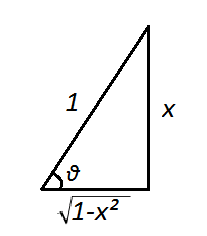
\includegraphics[width=0.25\textwidth]{images/b1p2-344-fig01}
	\centering
	sin Triangle\footnote{wrapfig package is used}
	\caption{}\label{wrap-fig:1}
\end{wrapfigure}
{
	\begin{sltn}
		Since square root is not involved, $1-x^2 > 0$ follows
		and the substitution $x = sin \theta $ may work
		$$I = \int \frac{cos \theta ~d\theta}{(1-sin^2\theta)^{3/2}}
		=\int \frac{cos \theta ~d\theta}{cos^3\theta}
		=\int sec^2\theta ~d\theta
		=tan\theta + c$$
	\end{sltn}
	\par
	The result is to be written in terms of x.
	Using the relation $x = sin \theta$ we have
	$$I = tan\theta + c = \frac{x}{\sqrt{1-x^2}} + c$$

\begin{exmp}
	Evaluate
	$$I = \int (x^3-2x+3)^{15}(3x^2-2)~dx$$\\
	\\
\end{exmp}
\begin{sltn}
	Observing that, $D(x^3-2x+3) = (3x^2-2)$ the proper
	substitution is $$u = (x^3-2x+3)\;\textrm{,} \quad du = (3x^2-2)~dx$$
\end{sltn}

% =======================================================
\end{document}  
